\chapter{Data Analysis}

\MyQuote{In physics, you don't have to go around making trouble for yourself - nature
does it for you.}{Frank Wilczek}

QCD jets are the most common hard objects observed in inelastic collisions 
at hadron colliders, with their cross section exceeding any other
physics process by orders of magnitude.  Measurement of the inclusive jet cross
section provides the test for both the QCD predictions and the detector
performance up to the momentum transfers not reachable by any other physics
processes. 

In this Chapter, I will describe the details of the double differential
inclusive jet cross section analysis, which I have performed in this thesis.
I will begin with the characteristics of the Monte Carlo sample, I have used.
This data together with the event selection criteria and matching procedure,
which description will follow, fully specify the input for the unfolding
procedure. Two approaches to the unfolding, which I have implemented in this
thesis, will be described and compared with each other. 

At the end of this Chapter, I will compare the results of my data analysis, with
the next-to-leading order perturbative QCD prediction of my supervisor. 

\section{Data Characteristics}

As the input, I have used Monte Carlo generated events of proton-proton collisions at
the center-of-mass energy $\sqrt{s} = 13\TeV$ with \textsc{Pythia8}
\cite{Pythia8} event generator using CT10 Parton Distribution Functions
\cite{CT10PDF} and ATLAS Underlying Event Tune AU2 \cite{AU2}. QCD calculations
are performed only to the leading order in \textsc{Pythia8}, so the initial hard
scattering is always simulated as an $2\,\rightarrow\,2$ process. The response of
the ATLAS detector on these events was simulated with \textsc{Geant4}
\cite{Geant4} full detector simulation.

Particles were recombined into jets using anti-$k_t$ jet algorithm with
parameter $R=0.4$. There are particle jets, reconstructed from the
\textsc{Pythia8} output, which, further in this thesis, are denoted as the truth jets,
and, next to them, there are a reco jets, reconstructed from the output of
\textsc{Geant4} detector simulation from the ATLAS detector topological cell
clusters. In data, the truth jets are stored in the \texttt{AntiKt4TruthJets}
\texttt{JetContainer}, whereas the reco jets were extracted from the \texttt{AntiKt4LCTopoJets}
\texttt{JetContainer}.

The events were generated in a slices according to the leading truth jet $\pt$. These
samples differ in an event weight, which is for the whole event calculated as 

\begin{equation}
  \text{weight} = \frac{\text{(XS)} \cdot \text{(FE)} \cdot w_0}{\text{(\# events)}},
\end{equation}
with XS being cross-section, FE filter efficiency and $w_0$ additional weight
factor stored in \texttt{EventInfoAux} container. Concrete values for datasets used in
this thesis are given in Table~\ref{tab:JZXW}.  

\begin{table}
  \centering
  \begin{tabular}{|c|rcr|c|c|c|}
    \hline 
     JZ & \multicolumn{3}{|c|}{$\pt$ range (GeV)} & Cross-section (fb) & Filter Efficiency & \# events  \\ 
    \hline
    \hline
		 JZ0W &     0 & - &    20 & 7.8420e+13 & 9.7193e-01 & 3498000 \\ 
    \hline
		 JZ1W &    20 & - &    80 & 7.8420e+13 & 2.7903e-04 & 2998000 \\
    \hline
		 JZ2W &    80 & - &   200 & 5.7312e+10 & 5.2261e-03 & 500000  \\
    \hline
		 JZ3W &   200 & - &   500 & 1.4478e+09 & 1.8068e-03 & 499500  \\
    \hline
		 JZ4W &   500 & - &  1000 & 2.3093e+07 & 1.3276e-03 & 477000  \\
    \hline
		 JZ5W &  1000 & - &  1500 & 2.3793e+05 & 5.0449e-03 & 499000  \\
    \hline
		 JZ6W &  1500 & - &  2000 & 5.4279e+03 & 1.3886e-02 & 493500  \\
    \hline
		 JZ7W &  2000 & + &       & 9.4172e+02 & 6.7141e-02 & 497000  \\
    \hline 
  \end{tabular}
  \caption{The cross-sections (XS), filter efficiency (FE) and number of events
  for the JZ samples, which differ in the leading truth jet $\pt$ range.}
  \label{tab:JZXW}
\end{table}

I have calibrated reco jets using the \textsc{ApplyJetCalibration}
\cite{ApplyJetCalibration} library v3.28 with configuration 
\texttt{JES\_Prerecommendation2015\_Feb2015.config} and
calibration sequence \texttt{JetArea\_Residual\_EtaJES}. In next, the reco jets
denote the reco calibrated jets.

In the analysis, I am using jets with transverse momentum $\pt>15\GeV$ and
rapidity $|y|<4$. Analysis is made in double binning in $\pt$ and $|y|$, with
the bin edges being the same as those used in the analyzes from 2011/2012 \cite{Analysis2012},
which have chosen the binning in $\pt$ so that the bin width corresponds roughly
to twice the value of the $\pt$ resolution in that bin. At high $\pt$, the bin
width was also optimized for statistical uncertainty.

\begin{align}
  \pt = \, &15-20-25-35-45-55-70-85-100-116-134-152- \nonumber \\
        &172-194-216-240-264-290-318-346-376-408- \nonumber \\
        &442-478-516-556-598-642-688-736-786-838- \nonumber \\
        &894-952-1012-1076-1162-1310-1530-1992-2300- \nonumber \\
        &2800-3400-4100-5000-6000-7200 \GeV, \nonumber \\
  |y| = \, &0.0-0.5-1.0-1.5-2.0-2.5-3.0-3.5-4.0.
  \label{eq:Binning}
\end{align}

\section{Event Selection}

In this Section, I describe the selection and the matching criteria, I have used
in my analysis. The former is needed to cut those jets (or those events) off,
which were misinterpreted by the detector. By the later, the pairs, each
containing one reco and one truth jet, are created. This provide
the inputs for the unfolding procedure, which is the subject of the next
Section.

More details, including graphical display and numerical results for procedures
described in this Section, are given in Appendix~\ref{App:CutAndMatchingResults}.

\subsection{Jet Cuts}
\label{SubSec:JetCuts}

I have implemented four jet cuts, which description follows. First two of these
cuts are needed to remove the jets, with $\pt$ or rapidity $y$ out of used binning.
The objective of the remaining cuts is to remove the events, which were badly
reconstructed by the detector.

\begin{itemize}
  \begin{samepage}
  \item \textbf{$\mathbf{\pt}$ Cut}
  \\*
    Reco and truth jets with $\pt > 15 \GeV$ were kept.
  \end{samepage}

  \item \textbf{$\mathbf{y}$ Cut}
  \\*
    Reco and truth jets with $|y| < 4$ were kept.

  \item \textbf{Zero jet (0-jet) Cut}
  \\*
    Only those events, which has at least one reco and one truth jet, after the
    $\pt$ and $y$ cuts, are considered.
    
  \item \textbf{Leading Ratio (LR) Cut}
  \\*
    In this cut the reco and truth jets with the highest $\pt$ were used. If
    there was only one reco jet left, the ratio $LR = p_{T,leading}^{reco} /
    p_{T,leading}^{truth}$ was calculated. If there were two reco jets, instead
    of $p_{T,leading}^{reco}$, the average $\pt$ of two leading reco jets was
    calculated. If $0.6 < LR < 1.4$ the event is considered.

\end{itemize}

Numbers of reco and truth jets, removed in each step, are shown in
Table~\ref{tab:CutAndMatchingEfficiency}, where also the cut efficiencies for
individual JZ samples are shown. The impact of each cut on the jet $\pt$ spectra
of reco and truth jets is displayed in Figure~\ref{fig:Cutting}. 

It can be seen, that the most important cut is the 0-jet cut, which removes
approximately $80\,\%$ of reco jets in JZ0W sample, whereas the truth jets
remain intact. According to Table~\ref{tab:JZXW}, the leading truth jet $\pt <
20 \GeV$ for event from the JZ0W sample, which has no longer to hold for reco
jets, which were, in some cases, reconstructed with $\pt \sim 100 \GeV$. Because
of Monte Carlo event weight for events from JZ0W sample is dominant over event
weights of other JZ samples by several orders, the misreconstructed reco jets
from JZ0W sample were negatively influencing the observed $\pt$ spectrum of reco
jets, as can be seen from top of the Figure~\ref{fig:Cutting}.

\subsection{Jet Matching}
\label{SubSec:JetMatching}

To find, how the truth jets are reconstructed by the detector, the jet matching
has to be performed, i.e. for each truth jet it is needed to find the corresponding reco
jet. In this thesis, I have used the matching based on the minimal angular distance
between matched jets.

For each pair $(i,j)$ of reco and truth jets, the quantity $dR_{ij} =
\sqrt{d\phi_{ij}^2 + dy_{ij}^2}$ was calculated, with $d\phi_{ij}$ being the angle
between $\phi_i^{reco}$ and $\phi_j^{truth}$ and $dy_{ij} = y_i^{reco} -
y_j^{truth}$.  The minimum was found between all of $dR_{ij}$'s. If this was
smaller than the defined cutoff $\min(dR_{ij}) = dR_{pq} < dR^{cutoff} = 0.2$,
the jets $(p,q)$ were matched and further not assumed in the matching procedure.
This continued until the condition $\min(dR_{ij}) < dR^{cutoff}$ was not satisfied
or all of the reco or truth jets were matched.

Numbers of reco and truth jets, both matched and unmatched, are shown in
Table~\ref{tab:CutAndMatchingEfficiency}, where also the matching efficiencies
for individual JZ samples are shown. Figure~\ref{fig:Matching} shows the $\pt$
spectra of truth and reco jets after event selection, which are composed from
$\pt$ spectra of matched and unmatched jets, which are in the
Figure~\ref{fig:Matching}  shown also.  $\pt$ spectra of truth and reco jets are
for all rapidity bins, assumed in this thesis, shown in
Figure~\ref{fig:ptSpectraMasacreEverythingFuck}.

\begin{figure}[t]
  \centering
  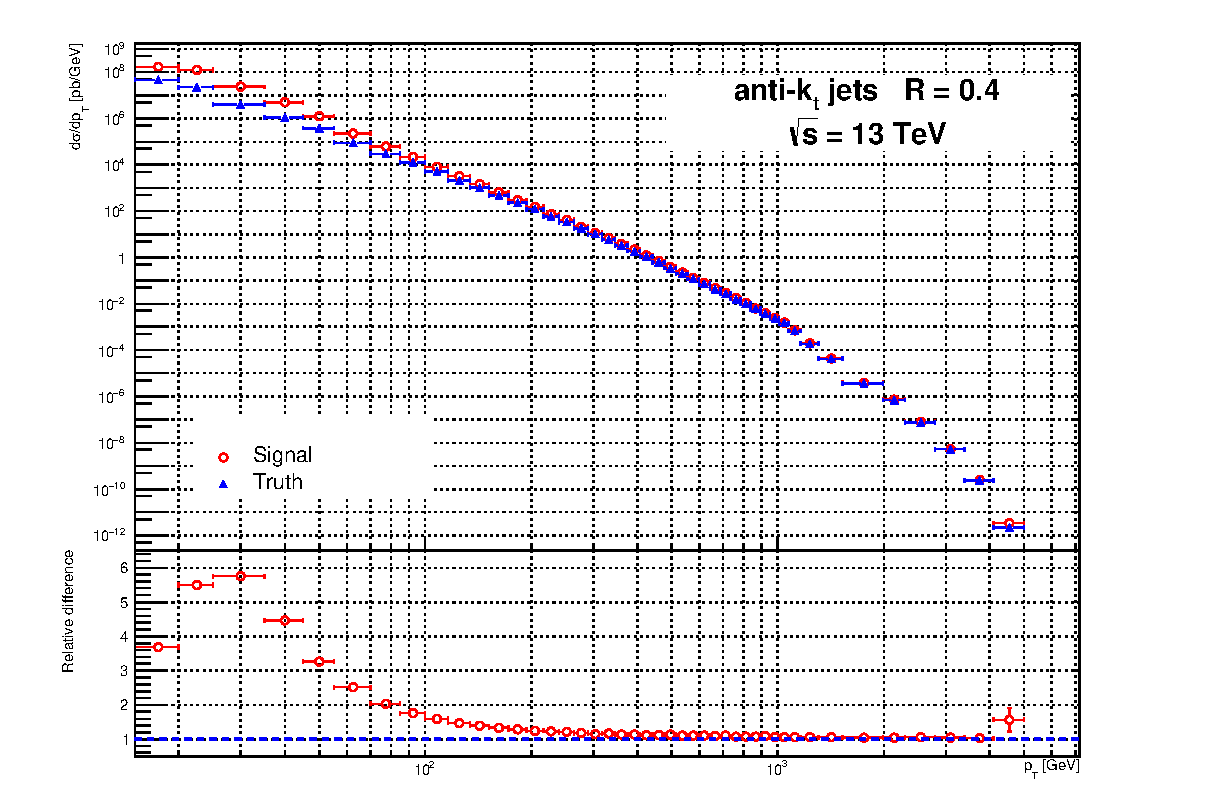
\includegraphics[width=\textwidth]{{Chapter3/SignalVSTruth}.eps}
  \caption{Comparison of $\pt$ spectra of reco and truth jets, after the event
    selection, for the $|y|<0.5$ rapidity bin. Each $\pt$ bin was divided by
    its width, so $y$-axis has physical meaning of double differential cross
    section in $\pt$ and $y$. Bottom graph contains the relative difference
    between reco and truth spectra.} 
  \label{fig:SignalVSTruth}
\end{figure}

\begin{figure}[p]
  \centering
  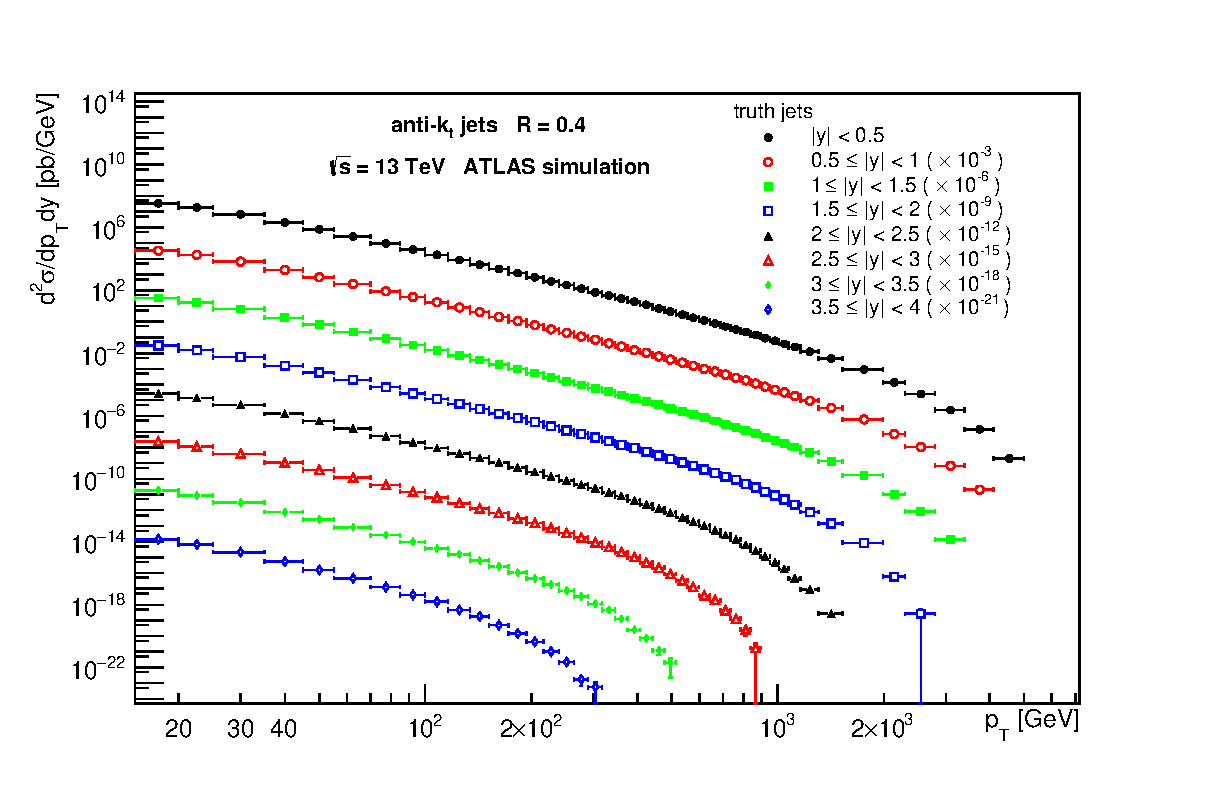
\includegraphics[width=\textwidth]{Chapter3/ptTruthAllRapidityBins.eps}
  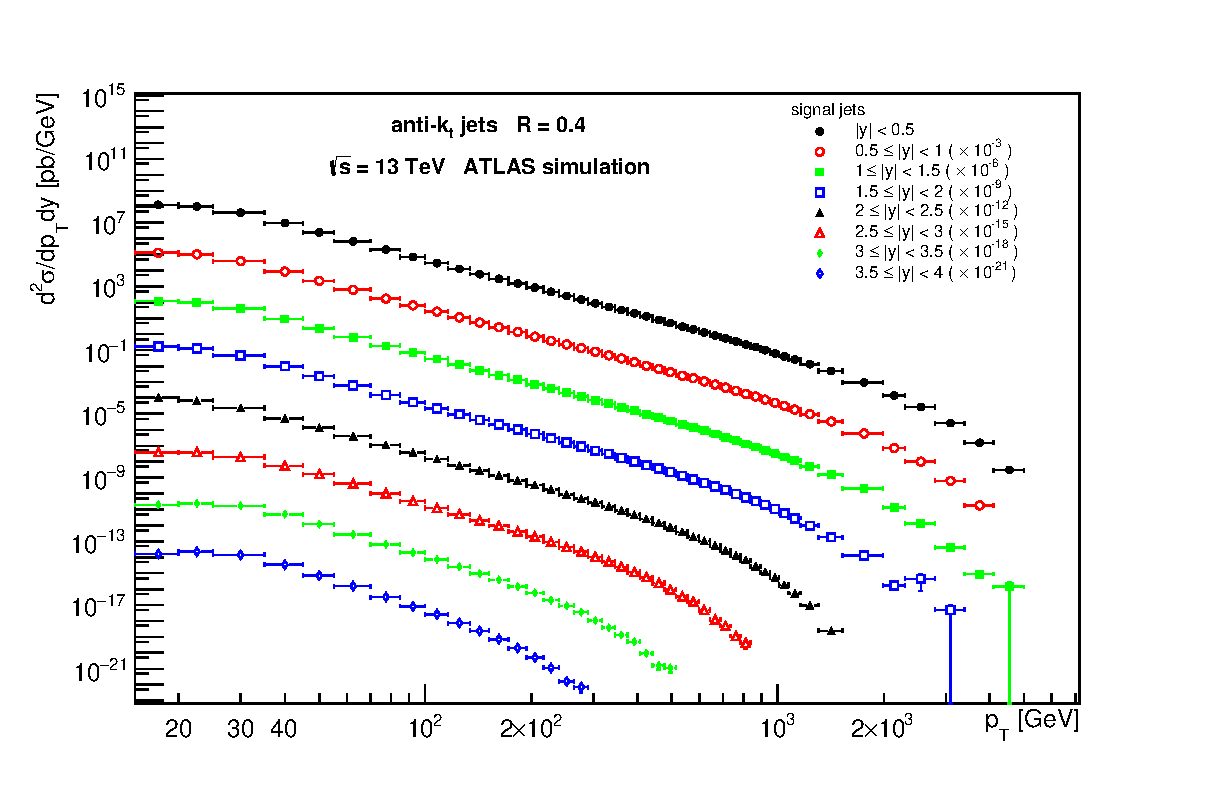
\includegraphics[width=\textwidth]{Chapter3/ptSignalAllRapidityBins.eps}
  \caption{Double differential inclusive jet cross section of truth (top) and
    reco (bottom) jets in $\pt$ and rapidity $y$.  For the convenience the cross
    sections for different rapidity bins are multiplied by the factor indicated
    in the legend. Jets were identified with the anti-$k_t$ jet algorithm with
    $R=0.4$.}
  \label{fig:ptSpectraMasacreEverythingFuck}
\end{figure}

\section{Unfolding}
\label{Sec:Unfolding3}

After the four cuts from the Section~\ref{SubSec:JetCuts}, the sets of jets,
denoted reco and truth jets, were obtained. The matching procedure, described in the
Section~\ref{SubSec:JetMatching},
divided both reco and truth jets into two categories, depending on successful
matching - there is correspondence 1 : 1 between matched reco and matched truth
jets. Reco jets, which were not matched, formed the unmatched reco jets, and,
similarly, the set of unmatched truth jets was created. All these 6 sets of jets
are needed by the unfolding procedure, which I describe in this Section.

From the Figure~\ref{fig:SignalVSTruth}, which shows the $\pt$ spectra of reco and
truth jets, it can be seen, that observed $\pt$ spectrum, represented by the reco jets,
differs from the $\pt$ spectrum theoretically expected, which is represented by
the $\pt$ spectrum of truth jets. The reason is, that the detector resolution is
folded into the reco spectra. Unfolding should transform the observed $\pt$
spectrum to the spectrum theoretically expected. If this transformation would be
done on real data, it should, ideally, preserve additional structures, which are
presented in data, but not included by the theory.

The main ingredient for the unfolding procedure is the transfer matrix $A_{ij}$,
which contains the number of reco jets in bin $i$ with a matched truth jets,
which was generated in bin $j$, and describes thus the smearing effects of the
detector. In this thesis, I use the double binning \eqref{eq:Binning}, which
complicates the situation, because the matched reco jet can simply migrate of the
transfer matrix from Figure~\ref{fig:UnfoldingMatrixDetail}, when, for example,
its rapidity $|y|>0.5$ and when it was matched with a truth jet with $|y|<0.5$ or
vice versa. In this thesis, I test two unfolding approaches, which offer
the dealing with double binning.

\begin{enumerate}
  \item \textbf{Simple unfolding}
  \\*
    In this case, only those reco and truth jets are used in the transfer
    matrix, which were matched within the same rapidity bin. Remaining matched
    jets are added to the unmatched jets. Eight transfer matrices $46 \times
    46$ are filled (one for each rapidity bin, $46$ = number of $\pt$ bins) and
    unfolding is done for each of these matrices separately. One of these
    matrices, for $|y|<0.5$ rapidity bin, is shown in
    Figure~\ref{fig:UnfoldingMatrixDetail}.

  \item \textbf{2D unfolding}
  \\*
    In this case, the unfolding matrix is redefined, to encapsulate the matching
    of jets between different rapidity bins. In this case, only one transfer
    matrix $368 \times 368$ is created ($368 = 46 \times 8$), with unfolding being
    done only for this matrix, shown at Figure~\ref{fig:UnfoldingMatrixAll}, from which
    the way, how the transfer matrix was redefined from the simple unfolding
    approach, should follow. 
\end{enumerate}

\begin{figure}[p]
  \centering
  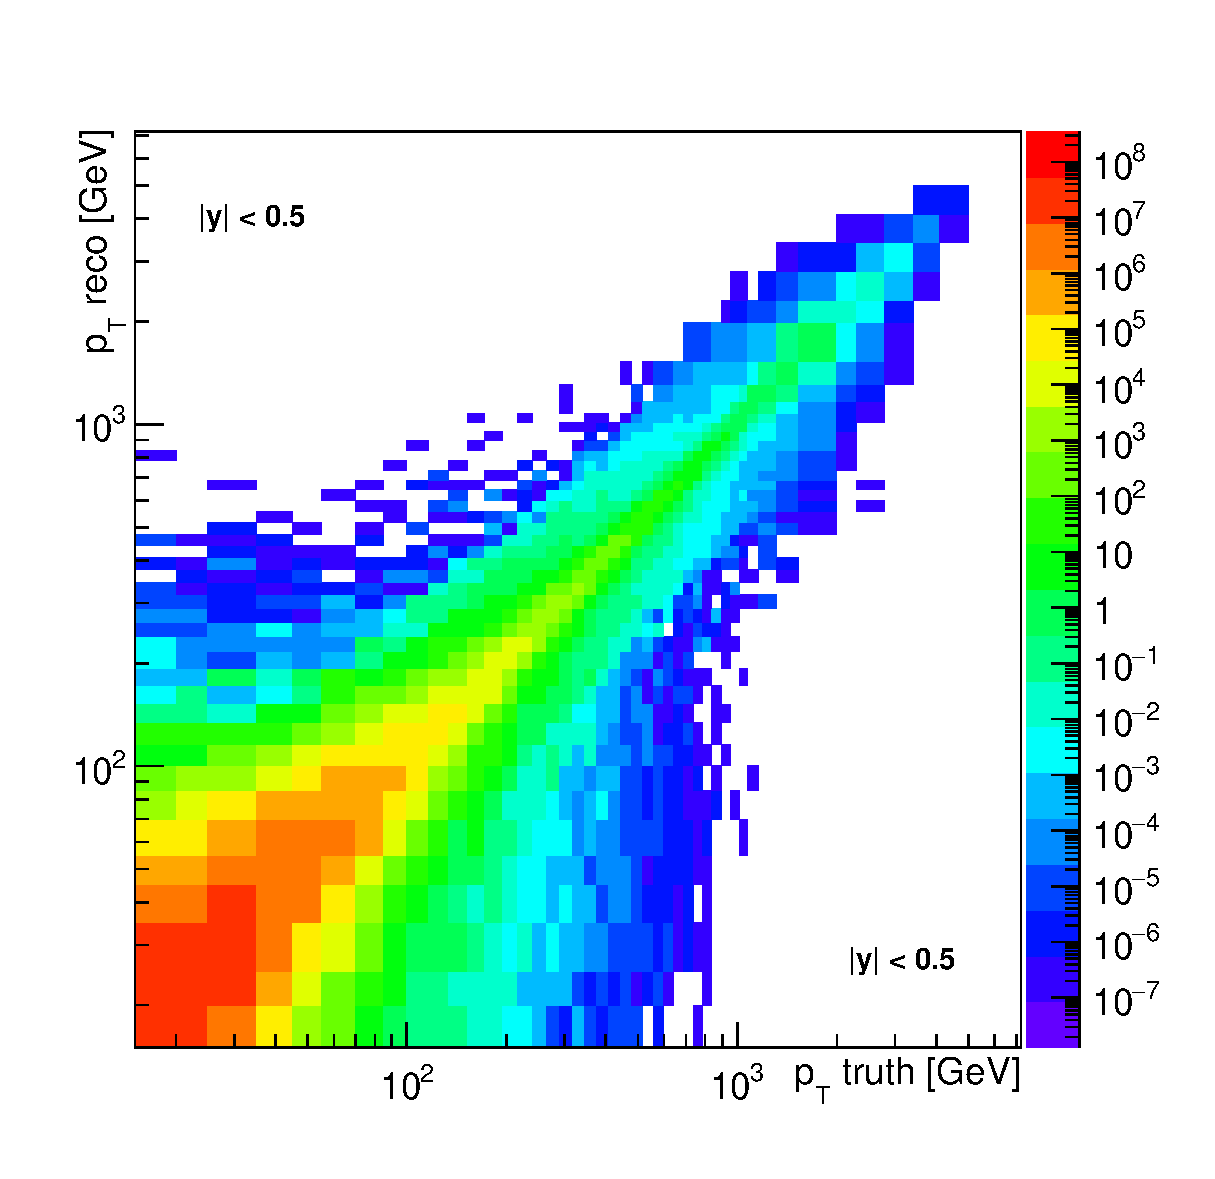
\includegraphics[width=\textwidth]{{Chapter3/Unfold_matrix_firstBin}.eps}
  \caption{Unfolding matrix for matched reco and truth jets with rapidity
  $|y|<0.5$, corresponding to one of eight transfer matrices used by the simple unfolding
  approach.  Each cell is proportional to the number of jets with truth $\pt$ in
  range determined by the $x$-axis, which were reconstructed to the reco jets
  with $\pt$ determined by the $y$-axis. White space signalize no input.}
  \label{fig:UnfoldingMatrixDetail}
\end{figure}

\begin{figure}[p]
  \centering
  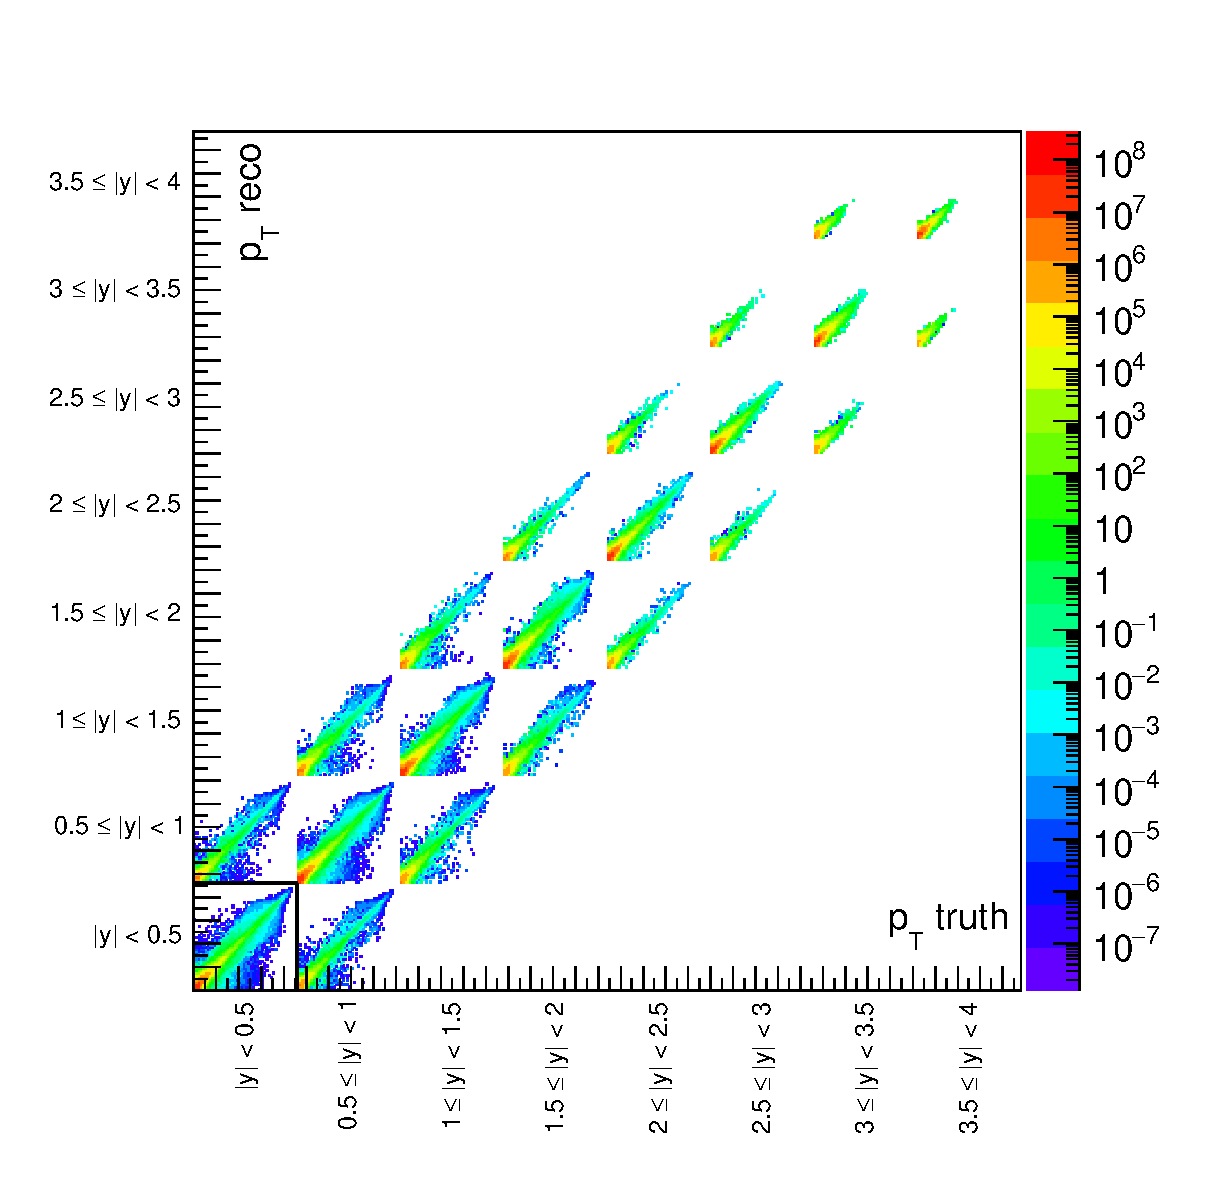
\includegraphics[width=\textwidth]{{Chapter3/Unfold_matrix_all}.eps}
  \caption{Transfer matrix used by the 2D unfolding approach. Each cell is
    proportional to the number of jets with truth $\pt$ and rapidity $y$
    determined by the $x$-axis, which were reconstructed to the reco jets with
    $\pt$ and $y$ determined by the $y$-axis. Marked square in $|y|<0.5$ region
    is the matrix shown in Figure~\ref{fig:UnfoldingMatrixDetail}. Projection of
    this matrix on the $x$ and $y$-axis corresponds to the $\pt$ spectrum of
    matched truth and reco jets for corresponding rapidity bin respectively.
    For better understanding of structure of this matrix, I have created some
    slices, which are shown in Appendix~\ref{sec:UnfoldingMatrixSlices}.} 
  \label{fig:UnfoldingMatrixAll}
\end{figure}

Transfer matrix from Figure~\ref{fig:UnfoldingMatrixAll}, used by the 2D
unfolding approach, contains 8 submatrices at the diagonal, which are the transfer
matrices used by the simple unfolding approach. Next to these submatrices,
the transfer matrix of the 2D unfolding approach contains 14 additional submatrices
beside the diagonal. These correspond to the matched jets with migration in
rapidity bins, and in case of simple unfolding approach, these jets are assumed to be
unmatched. 

It can be seen, from the slices from the
Appendix~\ref{sec:UnfoldingMatrixSlices}, that the dominant elements of each of
the submatrices are on the main diagonal, which correspond to the fact, there is
no significant bias in $\pt$ reconstruction.  The finite $\pt$ resolution causes
the smearing off the diagonal and a finite rapidity resolution is the cause of
the presence of 14 minor submatrices. Next it can be seen, that the elements
of the minor submatrices are approximately two orders in magnitude smaller, than
the corresponding submatrix on the main diagonal. This means, that the migration
of matched jets in rapidity is much smaller, than the migration in $\pt$. 

Next to the transfer matrix, numbers of matched and unmatched reco and truth
jets are needed, for each $(y,\pt)$ bin, by unfolding procedure. These serve for
calculation of matching efficiencies, which are the key ingredient in the first and
in the last step of the unfolding procedure. Matching efficiencies, for $|y|<0.5$
rapidity bin, are for both simple and 2D unfolding shown in
Figure~\ref{fig:MatchingEfficiencyDemonstration} and for other rapidity bins,
they are shown in Appendix~\ref{sec:MatchingEfficiency}.

\begin{figure}[p]
  \centering
    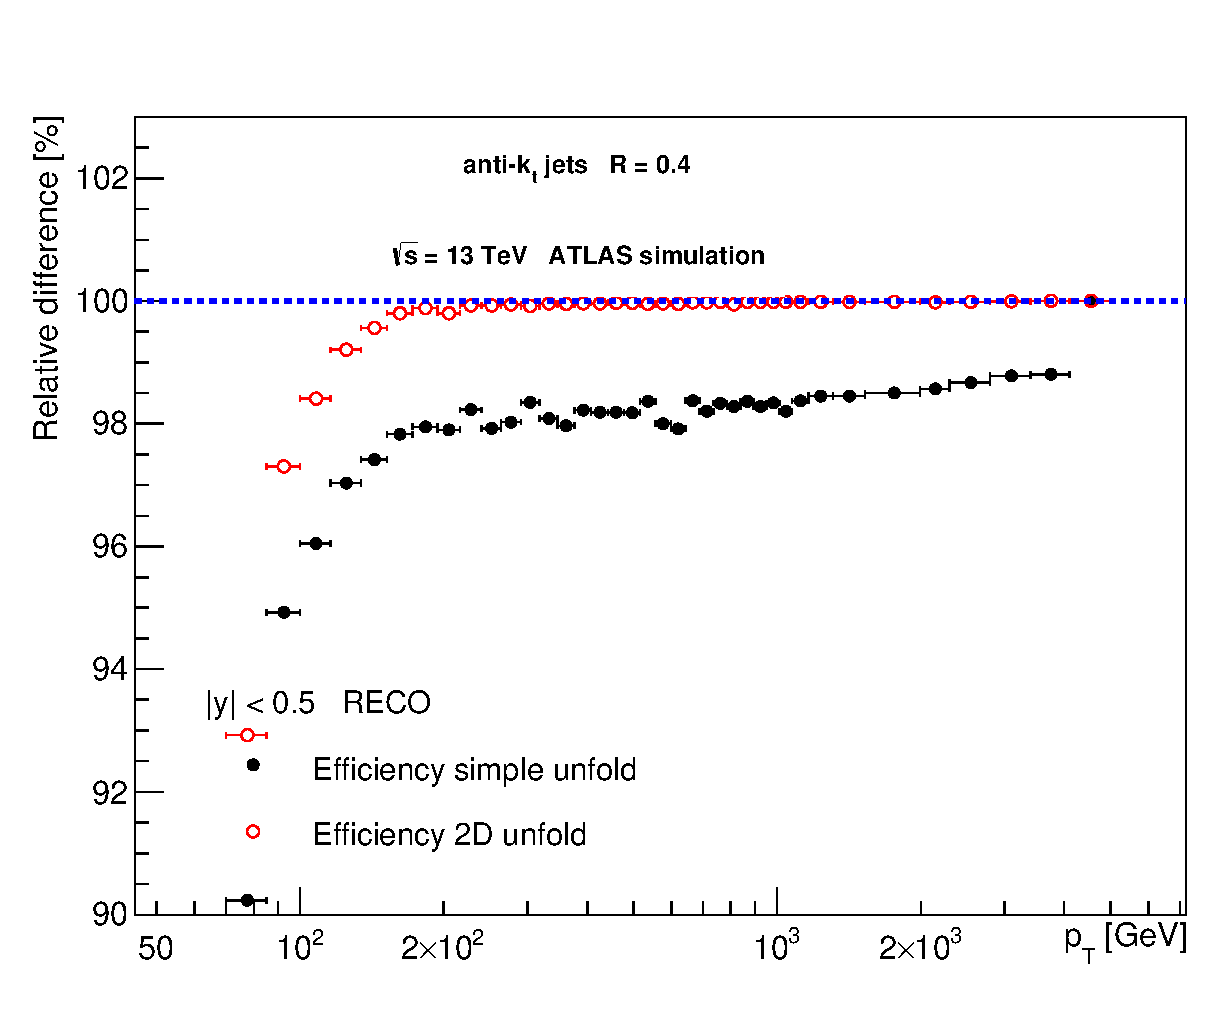
\includegraphics[width=0.49\textwidth]{{Chapter3/MatchEffSimpe2DSignal0Compare}.eps}
    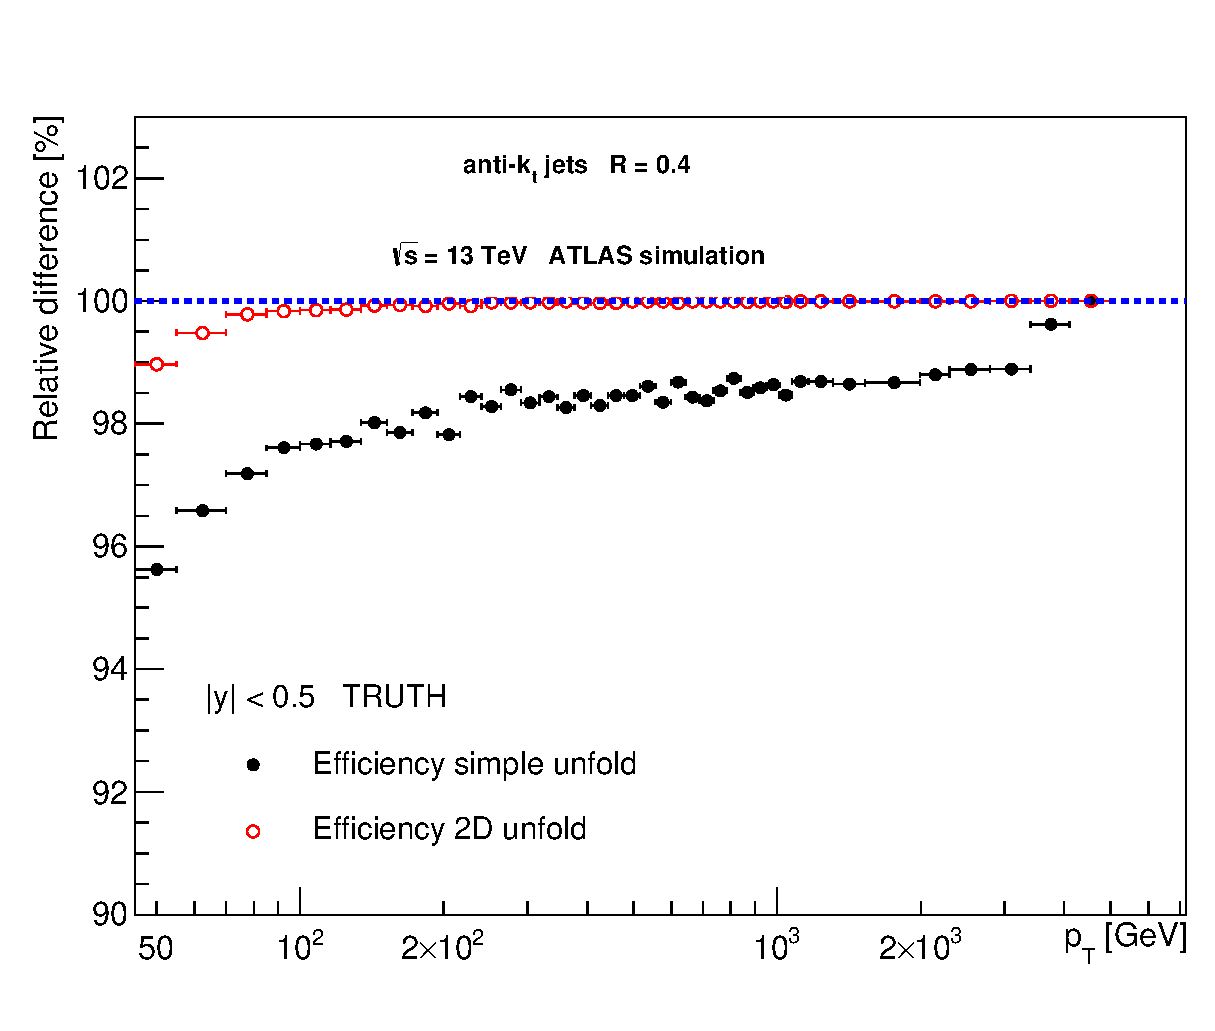
\includegraphics[width=0.49\textwidth]{{Chapter3/MatchEffSimpe2DTruth0Compare}.eps}
  \caption{Comparison of matching efficiencies of simple and 2D unfolding
    approaches for $|y|
    < 0.5$ rapidity bin. Matching efficiencies are compared for both reco jets
    (left) and truth jets (right). Matching efficiencies for all rapidity bins
    are shown in Appendix \ref{sec:MatchingEfficiency}.}
  \label{fig:MatchingEfficiencyDemonstration}

  \vspace{1cm}
  
    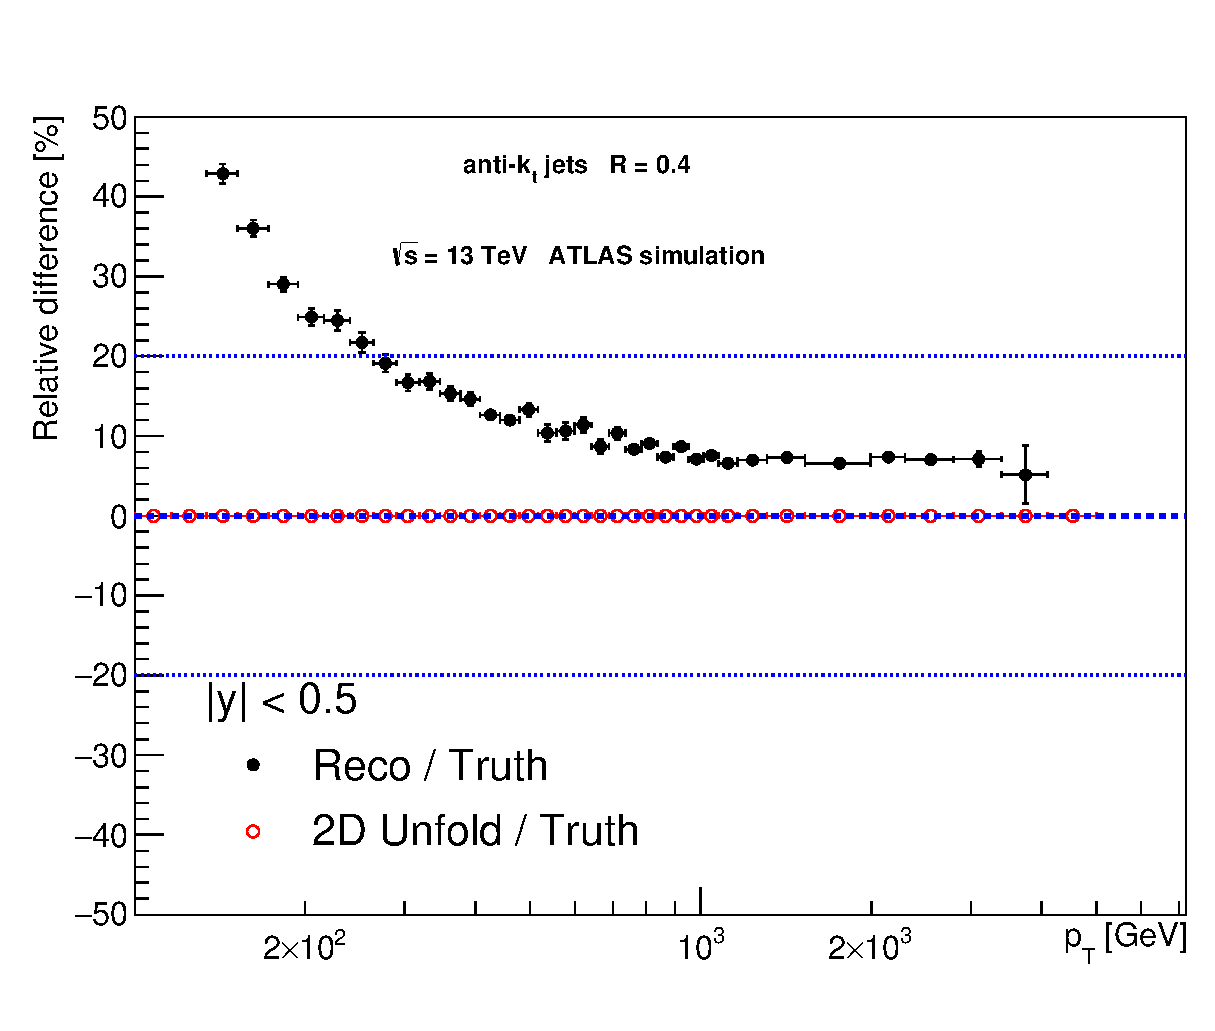
\includegraphics[width=0.49\textwidth]{{Chapter3/SignalUnfolded_VS_Truth0Compare}.eps}
    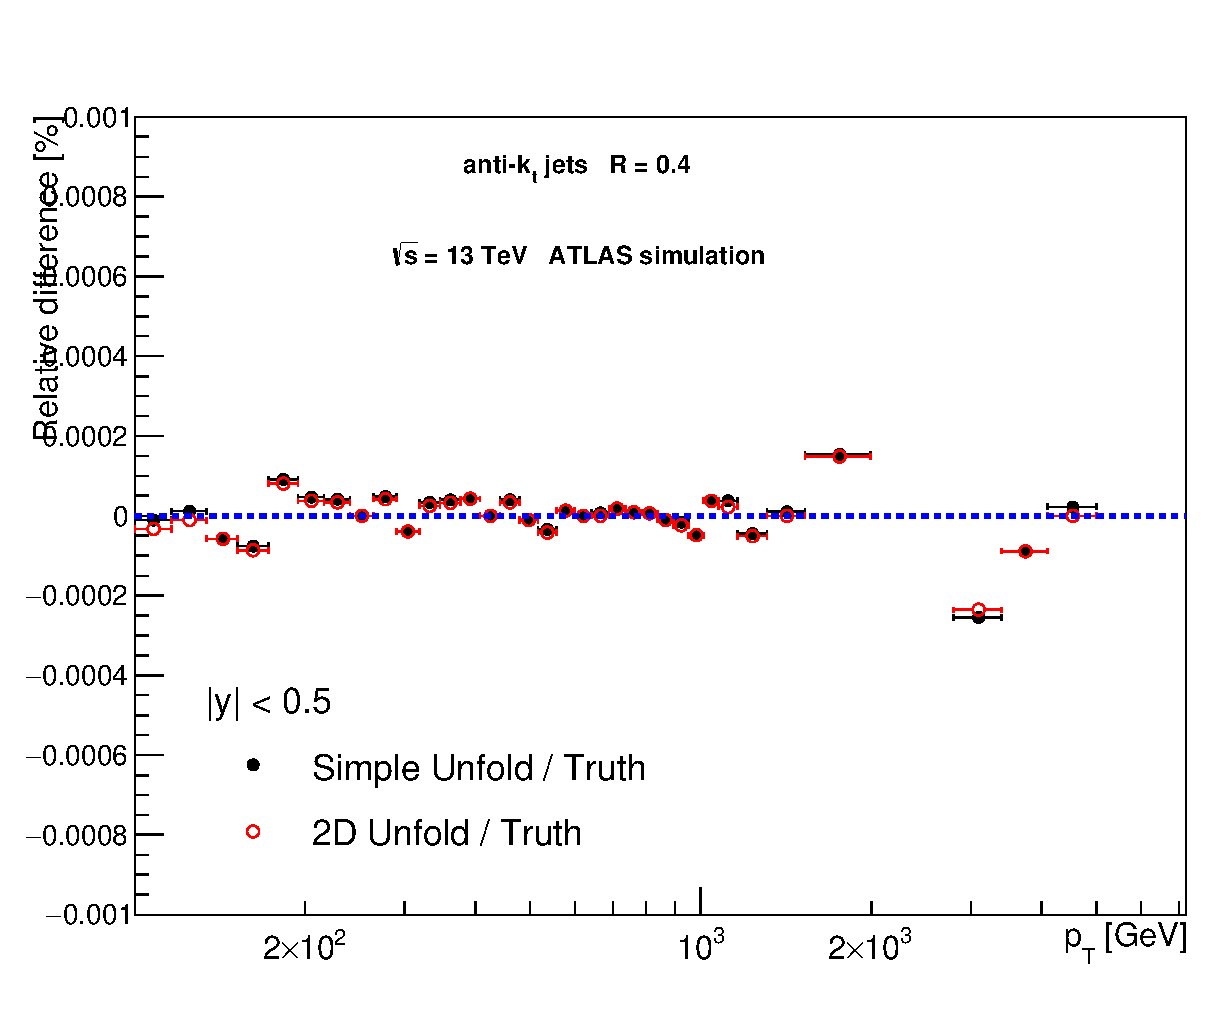
\includegraphics[width=0.49\textwidth]{{Chapter3/UnfoldedSimpleComplex_VS_Truth0Compare}.eps}
  \caption{Comparison of $\pt$ spectra of reco jets and the unfolded
    $\pt$ spectra (2D unfolding approach) with the $\pt$ spectra of truth jets
    on the left. The graph on the right shows the comparison of unfolded
    spectra, obtained by the 2D and simple
    unfolding approaches, with the $\pt$ spectra of truth jets. Both graphs are
    for $|y|<0.5$ rapidity regions. Results for all rapidity bins are shown in
    Appendices \ref{sec:UnfoldingResults}, \ref{sec:SimpleAnd2DUnfolding}. }
  \label{fig:UnfoldingResultsDemonstration}
\end{figure}


Unfolding procedure can be divided into three main steps

\begin{enumerate}
  \item Input data are multiplied by the matching efficiencies of reco jets.
  \item Transfer matrix is used to correct data spectrum for detector effects.
    For this purpose, the Iterative Dynamical Stabilized (IDS)
    \cite{IterativeDynamicallyStabilized} unfolding method was implemented,
    which uses the series of iterations to improve unfolding results. In this
    thesis, I have performed just one iteration.
  \item The spectrum obtained by the step 2 is divided by the matching
    efficiencies of truth jets, in order to correct resulting spectrum for the
    unmatched truth jets.
\end{enumerate}

Figure~\ref{fig:UnfoldingResultsDemonstration} shows, on the left, the comparison of $\pt$
spectra of reco jets and unfolded spectra (by 2D unfolding approach) with the
$\pt$ spectra of truth jets on the left. The right part of the
Figure~\ref{fig:UnfoldingResultsDemonstration} contains the comparison of simple and 2D unfolded
spectra with the spectrum of truth jets for $|y|<0.5$ rapidity bin.
Results for all rapidity bins are shown in Appendix~\ref{sec:UnfoldingResults}.

From figures it follows, that the unfolding procedure corrects the
$\pt$ spectrum of reco jets to $\pt$ spectrum of truth jets up to the systematic
error $<10^{-3}\,\%$ and that the differences between the results from simple and 2D
unfolding approaches are even smaller.

\section{Comparison with NLO Prediction}
\label{sec:ComaprisonWithNLOPrediction}

In the previous Sections, I have described the jet calibration and the unfolding
procedure. 
These serve to remove the ATLAS detector related effects, allowing corrected
$\pt$ spectrum of reco jets to be compared with a theory, as well as with other
experiments. The corrections were determined using the
events generated by \textsc{Pythia8}, which uses
the leading order QCD calculations to simulate the initial proton-proton collision.
Nowadays the QCD predictions are tested up to the next-to-leading order and for
LHC Run~II, new calculations, assuming the next-to-next-to-leading order QCD
processes, are in preparation \cite{NNLO1,NNLO2}.

My supervisor has calculated the theoretical prediction of $\pt$ spectra of
parton jets using \textsc{NLOJET++} program \cite{NLOJetProgram}. This
program computes the QCD processes up to next-to-leading order with CT10
parton distribution functions \cite{CT10PDF, Annecy}. In this thesis, I have used
his computations for center-of-mass energies $\sqrt{s}=8\TeV$ and
$\sqrt{s}=13\TeV$, the first corresponding to the LHC Run~I and the second to
the LHC Run~II. 

Firstly, I have compared the next-to-leading order predictions for two different
center-of-mass energies of proton-proton collisions.
The comparison is shown, for the $|y|<0.5$ rapidity region, in
Figure~\ref{fig:ComparePredictionsDemonstation}, where next to the double differential
cross section, the expected numbers of jets for the statistics of the LHC Run~I
and for expected statistics for the LHC Run~II are shown.
The numbers were obtained by multiplying each bin by its width in $\pt$ and
by the integrated luminosity of Run~I ($20\,\text{fb}^{-1}$) and expected
integrated luminosity of 
Run~II ($100\,\text{fb}^{-1}$) respectively. Comparisons for other rapidity bins
are shown in Appendix~\ref{sec:PredictionsForRunIAndII}.

\begin{figure}[t]
  \centering
  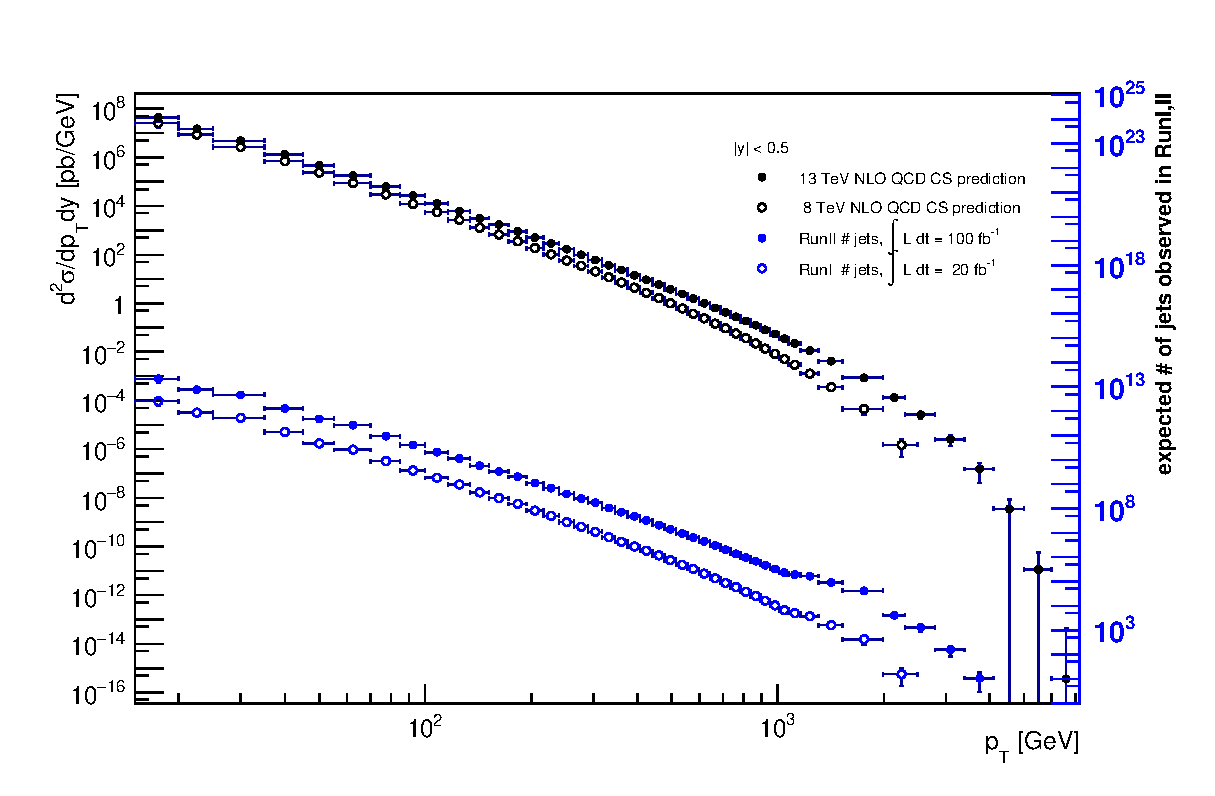
\includegraphics[width=\textwidth]{{Chapter3/PredictionCompare0}.eps} 
  \caption{Comparison of next-to-leading order QCD predictions of double differential inclusive jet
    cross section (black) for proton-proton collisions at $\sqrt{s}=13\TeV$
    (filled circles),
    corresponding to the LHC Run~II, and $\sqrt{s}=8\TeV$ (empty circles),
    corresponding to the LHC Run~I. The cross section is multiplied by
    integrated luminosities and bin width in $\pt$, to obtain the expected
    numbers of jets observed in each $\pt$ bin (blue). Figure shows only $|y|<0.5$ rapidity bin,
    remaining rapidity bins are shown in Appendix~\ref{sec:PredictionsForRunIAndII}.}
  \label{fig:ComparePredictionsDemonstation}
\end{figure}

It can be seen, that the increase in the center-of-mass energy is the most
significant for jets with high $\pt$. 

In the next-to-leading theoretical computations, several uncertainties are taken
into account. In this thesis, I assume the following uncertainties 

\begin{figure}[p]
  \centering
  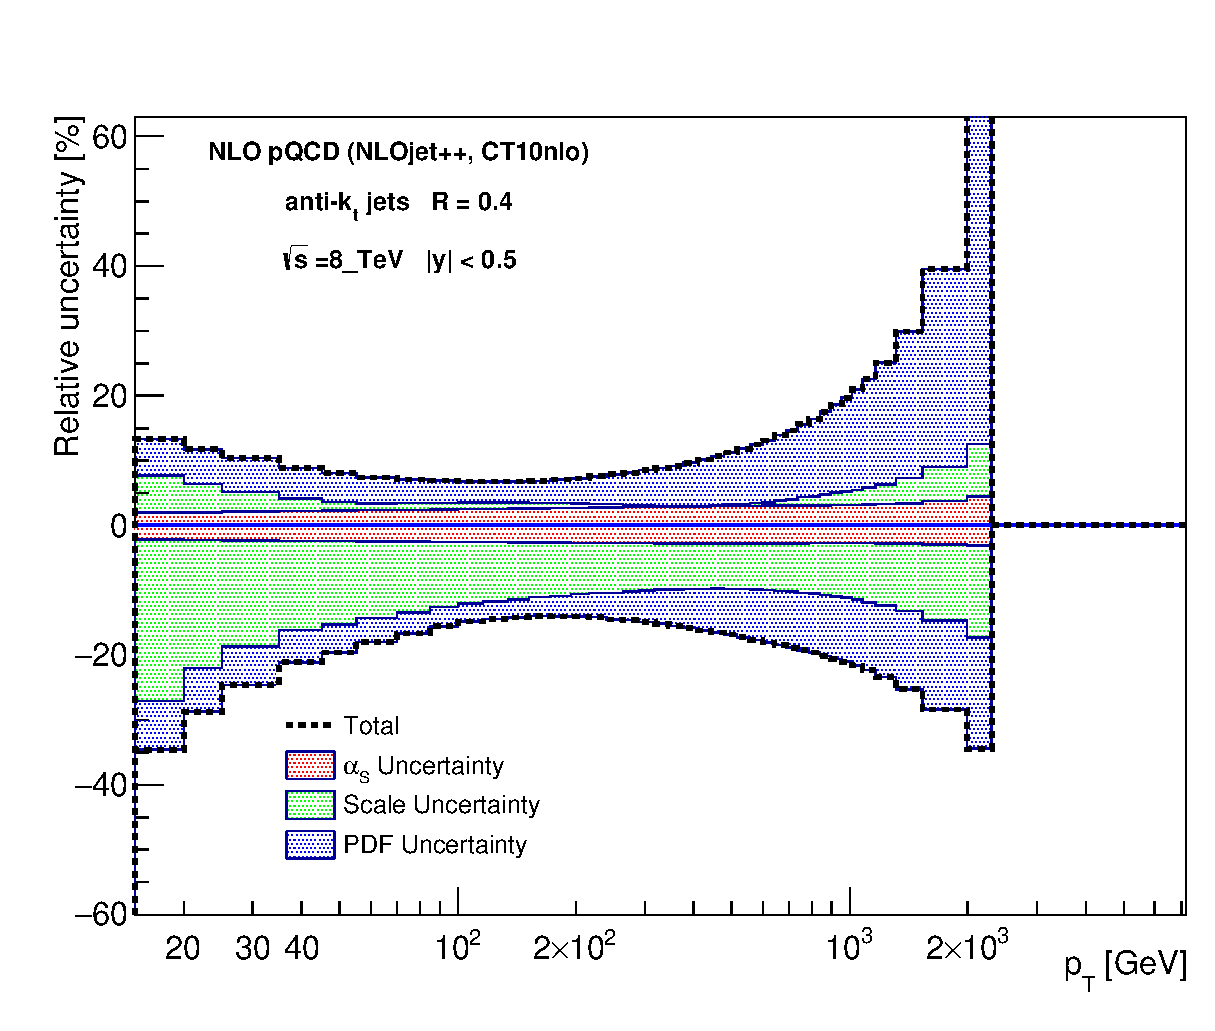
\includegraphics[width=0.8\textwidth]{{Chapter3/NLO_Systematics8_TeV0}.eps}
  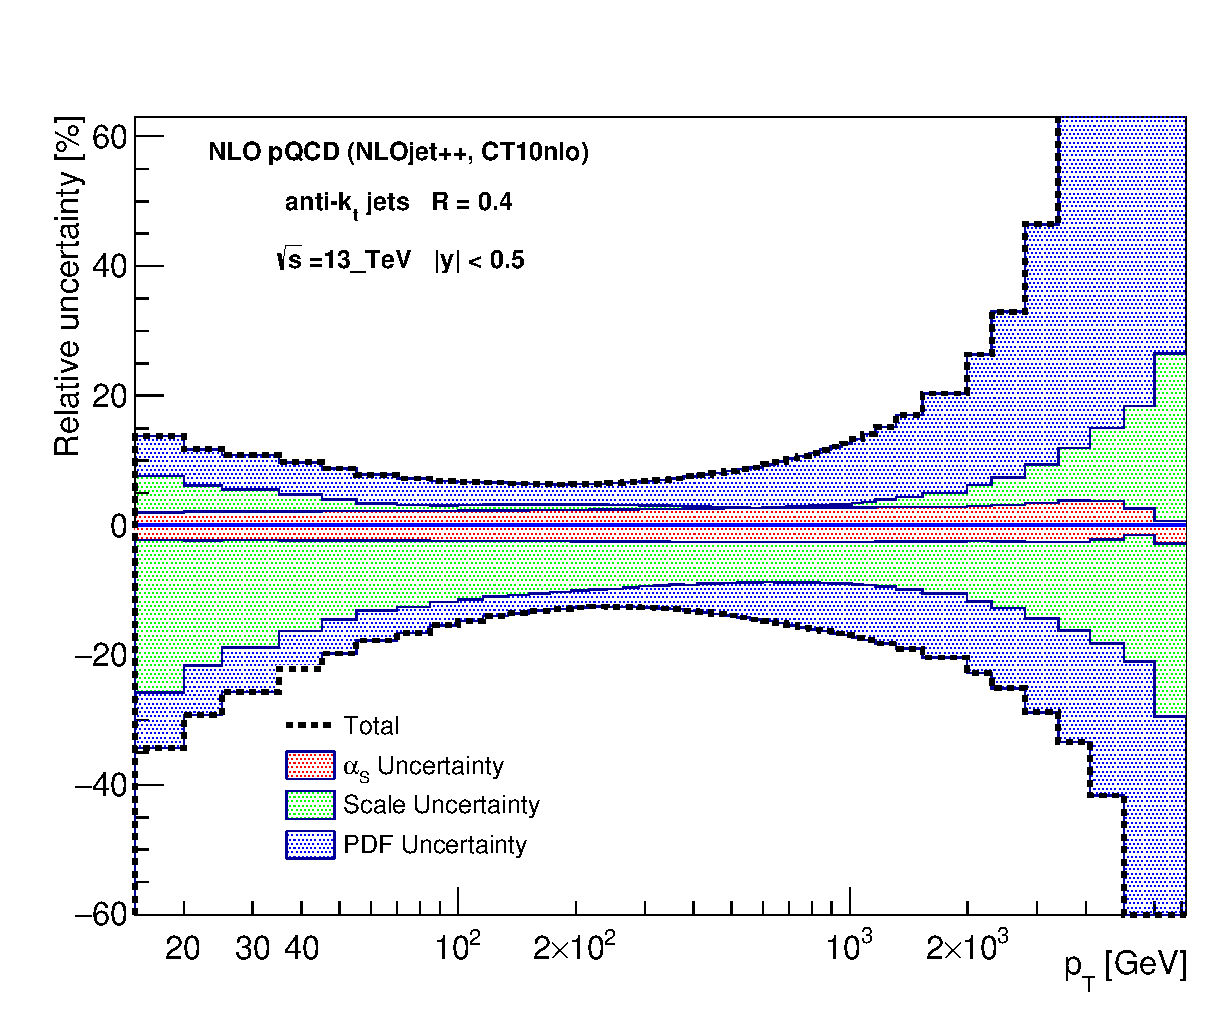
\includegraphics[width=0.8\textwidth]{{Chapter3/NLO_Systematics13_TeV0}.eps}
  \caption{Theoretical uncertainties for next-to-leading order QCD predictions
    of inclusive jet double differential cross section for proton-proton collisions at
    $\sqrt{s}=8\TeV$ (top) and $\sqrt{s}=13\TeV$ (bottom) for $|y|<0.5$ rapidity
    bin. Uncertainties for other rapidity bins are shown in
    Appendix~\ref{sec:NLOUncertainties}.}
    \label{fig:NLOSystematicsDemonstartion}
\end{figure}

\begin{itemize}
  \item \textbf{Scale uncertainty}
  \\*
    Coming from the choice of renormalization and factorization scales,
    including neglecting the higher order terms beyond the next-to-leading order 

  \item \textbf{$\alpha_S$ uncertainty}
  \\*
    Because of experimental measurements of $\alpha_S$.

  \item \textbf{PDF uncertainty}
  \\*
    Prediction depends on the concrete choice of a Parton Distribution Function.
\end{itemize}

Two uncertainties should be assumed, to correct the cross section from parton
level to particle level. According to the analysis from 2013
\cite{Analysis2012}, the corrections coming from these uncertainties are not as
significant as the three corrections mentioned already, and include

\begin{itemize}
  \item \textbf{Nonperturbative corrections uncertainty}
  \\*
    Hadronization and Underlying Event corrections.

  \item \textbf{Electroweak corrections uncertainty}
  \\*
    Next to the QCD processes, the electroweak processes has to be assumed.
    These processes becomes more important, as the momentum transfer
    increases.  
\end{itemize}


\begin{figure}[t]
  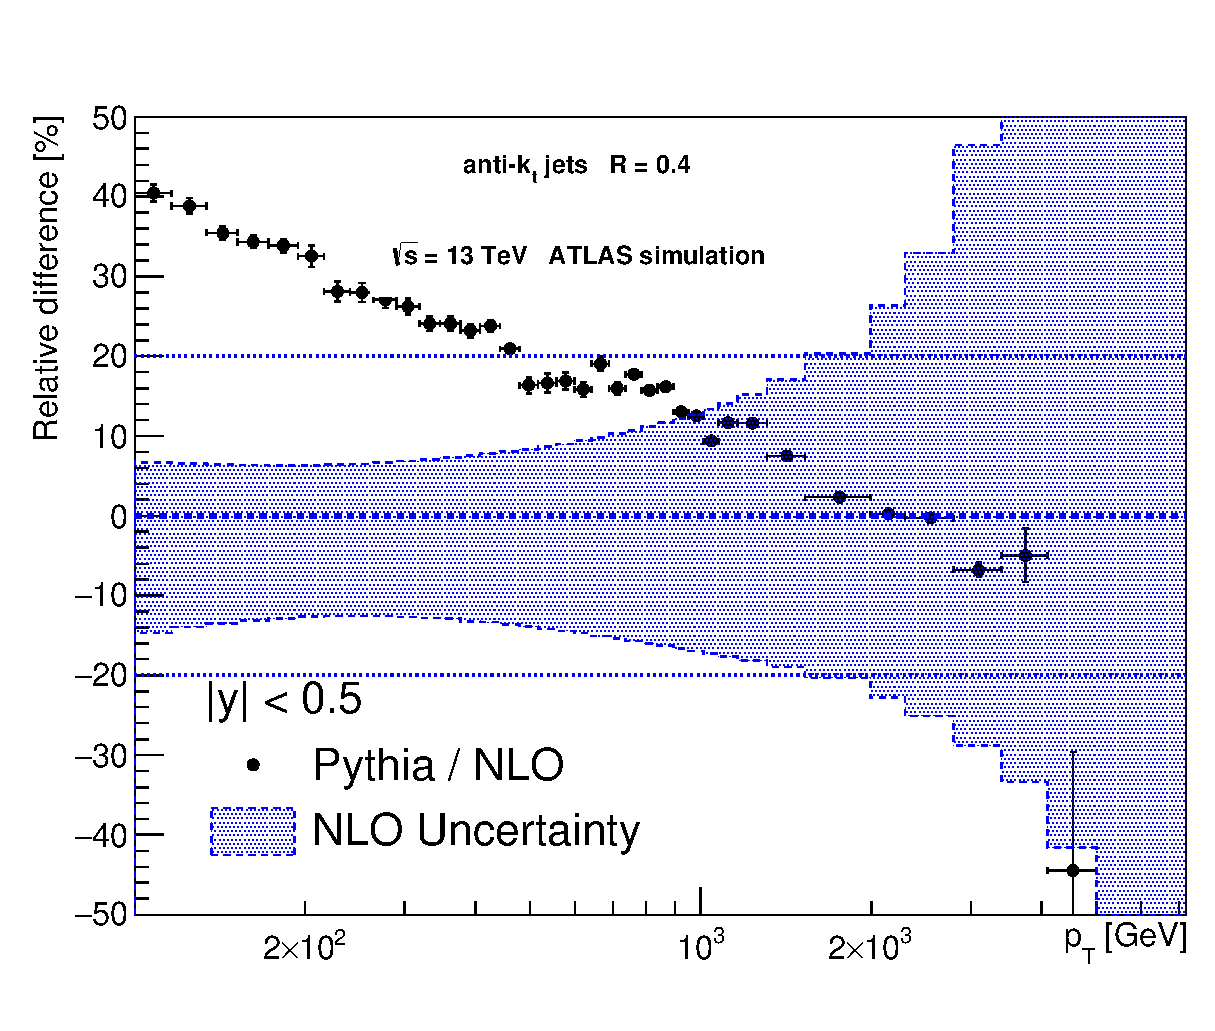
\includegraphics[width=\textwidth]{{Chapter3/Truth_VS_Prediction0Compare}.eps}
  \caption{Comparison of \textsc{Pythia8} prediction with next-to-leading order QCD prediction of
    inclusive jet double differential cross section for $|y|<0.5$ rapidity bin,
    with uncertainties of next-to-leading order QCD predictions symbolized by the blue area.
    Comparisons for other rapidity bins are shown in Appendix
    \ref{sec:PythiaAndNLO}.}
  \label{fig:TruthVSPredictionsDemonstation}
\end{figure}

The uncertainties were extracted from the files with the next-to-leading order QCD
predictions, where each correction is represented by the set of equally likely
histograms, expressing the deviation from the default prediction. Uncertainties
are, for $|y|<0.5$ rapidity bin, shown in
Figure~\ref{fig:NLOSystematicsDemonstartion}, other rapidity bins are shown in
Appendix~\ref{sec:NLOUncertainties}.

Comparison of $\pt$ spectra of truth jets with the next-to-leading order QCD
prediction is, for $|y| < 0.5$ rapidity bin, shown in
Figure~\ref{fig:TruthVSPredictionsDemonstation}, for other rapidity bins see
Appendix~\ref{sec:PythiaAndNLO}. It can be seen, that the
truth $\pt$ spectrum is for jets with low $\pt$ greater, then the next-to-leading order QCD
prediction, and that for a few $\pt$ bins with the highest $\pt$, the situation is
reversed. 

Generally, there is a significant difference between the leading order QCD
prediction, which I have extracted from the $\pt$ spectra of truth jets in
\textsc{Pythia8} generated events, and the next-to-leading order QCD prediction,
which my supervisor has calculated using the \textsc{NLOJET++} program. The
differences are greater then the theoretical uncertainties, successfully
demonstrating the influence of the next-to-leading order QCD processes on
observables.
